Let's review the output of the parametric run that we carried out:


% I will take 4 combinations of n_nodes and n_experiments



% n_nodes = 10
% n_experiments=4000
% iter = 5000

%n_nodes = 10 
% n_experiments=2000
% iter = 5000


%n_nodes = 30 
% n_experiments=4000
% iter = 5000

%n_nodes = 30 
% n_experiments=2000
% iter = 5000

% Please add the following required packages to your document preamble:
% \usepackage{multirow}
% Please add the following required packages to your document preamble:
% \usepackage{multirow}
\begin{table}[!hb]

\begin{minipage}{.49\textwidth}

\begin{tabular}{lllllllcc|ccc}
\multicolumn{9}{c|}{\multirow{2}{*}{\begin{tabular}[c]{@{}c@{}}$n_{nodes}=10$\\ $n_{experiments}=4000$\end{tabular}}} & \multicolumn{3}{c}{$n_{neurons}$} \\
\multicolumn{9}{c|}{}                                                                                                 & 10        & 20        & 40        \\ \hline
        &         &         &         &         &         &         & \multirow{4}{*}{\rotatebox{90}{$n_{layers}$}}        & 2        &  0.964        &  0.951        &  0.966        \\
        &         &         &         &         &         &         &                                      & 3        &  0.973        &  0.999       &  0.999        \\
        &         &         &         &         &         &         &                                      & 4        &  0.998        &  0.996        &  0.998        \\
        &         &         &         &         &         &         &                                      & 6        &  0.990       & 0.998       &  0.999      
\end{tabular}



\end{minipage}

\begin{minipage}{.49\textwidth}
\begin{tabular}{lllllllcc|ccc}
\multicolumn{9}{c|}{\multirow{2}{*}{\begin{tabular}[c]{@{}c@{}}$n_{nodes}=10$\\ $n_{experiments}=2000$\end{tabular}}} & \multicolumn{3}{c}{$n_{neurons}$} \\
\multicolumn{9}{c|}{}                                                                                                 & 10        & 20        & 40        \\ \hline
        &         &         &         &         &         &         & \multirow{4}{*}{\rotatebox{90}{$n_{layers}$}}        & 2        &  0.946        & 0.956         &  0.960        \\
        &         &         &         &         &         &         &                                      & 3        &  0.996        &  0.999        &  0.997        \\
        &         &         &         &         &         &         &                                      & 4        &  0.995        & 0.999         & 0.998         \\
        &         &         &         &         &         &         &                                      & 6        & 0.994         & 0.998         &  0.998       
\end{tabular}
\end{minipage}

\begin{minipage}{.49\textwidth}
\begin{tabular}{lllllllcc|ccc}
\multicolumn{9}{c|}{\multirow{2}{*}{\begin{tabular}[c]{@{}c@{}}$n_{nodes}=30$\\ $n_{experiments}=4000$\end{tabular}}} & \multicolumn{3}{c}{$n_{neurons}$} \\
\multicolumn{9}{c|}{}                                                                                                 & 10        & 20        & 40        \\ \hline
        &         &         &         &         &         &         & \multirow{4}{*}{\rotatebox{90}{$n_{layers}$}}        & 2        & 0.932         &   0.950       &  0.964        \\
        &         &         &         &         &         &         &                                      & 3        &  0.990        & 0.994         &  0.997        \\
        &         &         &         &         &         &         &                                      & 4        &  0.992        &  0.997        &  0.999        \\
        &         &         &         &         &         &         &                                      & 6        &  0.991        &  0.996       &        0.998 
\end{tabular}
\end{minipage}

\begin{minipage}{.49\textwidth}
\begin{tabular}{lllllllcc|ccc}
\multicolumn{9}{c|}{\multirow{2}{*}{\begin{tabular}[c]{@{}c@{}}$n_{nodes}=30$\\ $n_{experiments}=2000$\end{tabular}}} & \multicolumn{3}{c}{$n_{neurons}$} \\
\multicolumn{9}{c|}{}                                                                                                 & 10        & 20        & 40        \\ \hline
        &         &         &         &         &         &         & \multirow{4}{*}{\rotatebox{90}{$n_{layers}$}}        & 2        & 0.953         &  0.944        &  0.979        \\
        &         &         &         &         &         &         &                                      & 3        &  0.987        &  0.994        &  0.996        \\
        &         &         &         &         &         &         &                                      & 4        &  0.993        &  0.997        & 0.997         \\
        &         &         &         &         &         &         &                                      & 6        & 0.989         &  0.995        &  0.998       
\end{tabular}
\end{minipage}


\end{table}


The best configuration is a combination of 4 layers, 20 neurons, 2000 experiments, 10 nodes and 5000 iterations with an R2 on the test cases of 0.9994

Here is the output of the displacements predicted by the Neural Network compared against the FE outputs:

\begin{figure}
  \centering
  \subfloat[Displacement in the first axis of the coordenate system]{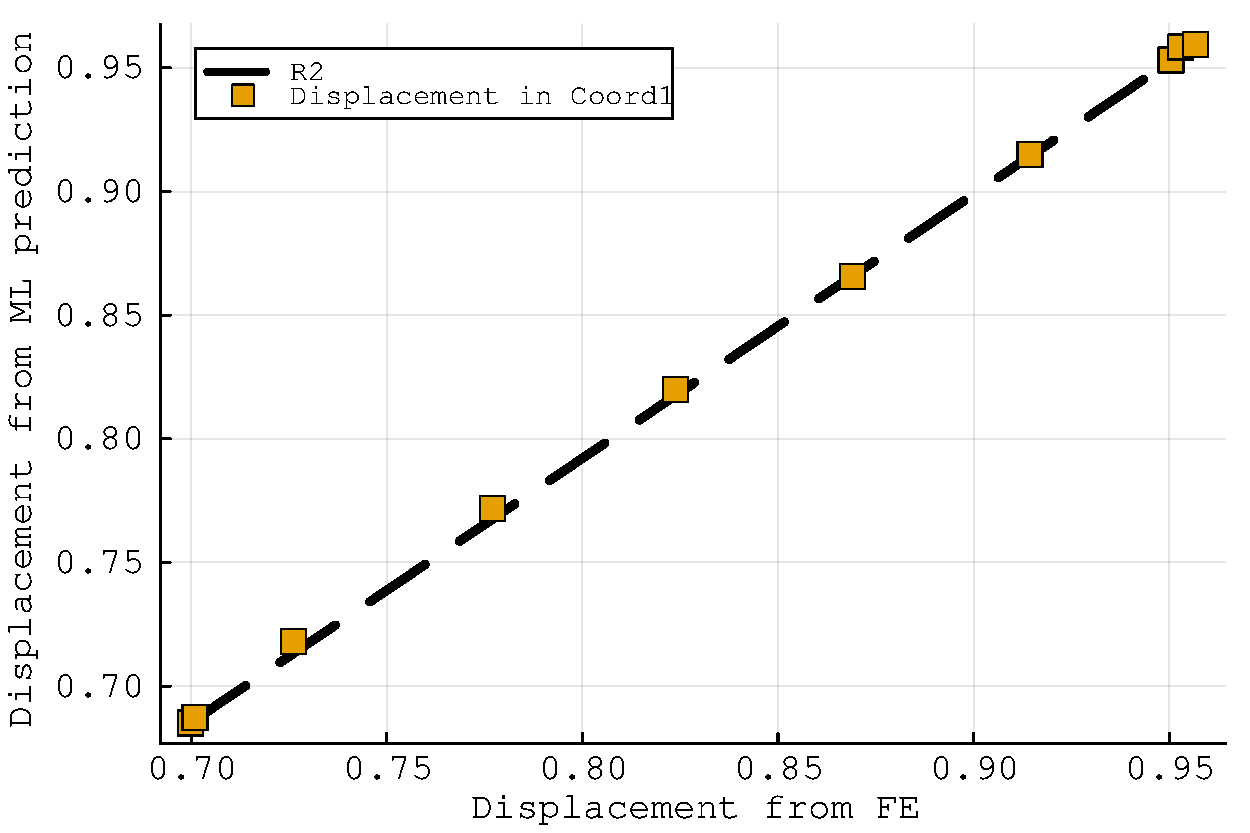
\includegraphics[width=0.45\linewidth]{Figures/NeuralNetworkStudy/R2_Coord1.pdf}}
  \subfloat[Displacement in the third axis of the coordenate system]{\includegraphics[width=0.45\linewidth]{Figures/NeuralNetworkStudy/R2_Coord3.pdf}}
  \caption{R2 evaluation of the displacements. FE data vs ML predicted output}
\end{figure}



Then, we can plot the loss function during the training to visualize the downward tendency.

\begin{figure}
  \begin{center}
    \includegraphics[width=0.6\textwidth]{Figures/NeuralNetworkStudy/Loss_1.pdf}
  \end{center}
  \caption{Loss function during the training for the best performant neural network configuration}\label{fig:}
\end{figure}


